\documentclass[oneside,a4paper,english,links]{article}
%
\usepackage{graphicx}
\usepackage{amsmath,amsfonts}
%\usepackage{fullpage}
\usepackage{url}
\usepackage{subfig}
\usepackage{ amssymb }

\newcommand{\rodrigo}[1]{\authnote{Rodrigo}{#1}}

\title{Bread Crumb classification using the sandbox multifractal method}

\author{Rodrigo Baravalle}

\begin{document}

\maketitle
\begin{center}
\small{Laboratorio de Sistemas Din\'amicos y Procesamiento de Informaci\'on, FCEIA, Universidad Nacional de Rosario - CIFASIS - CONICET}\\
\small{Riobamba 250 bis, 2000, Rosario, Argentina}\\

\texttt{baravalle@cifasis-conicet.gov.ar}\\
\texttt{\url{http://www.cifasis-conicet.gov.ar/index.php?grupo=4}}
\end{center}

\begin{abstract}
Adequate image descriptors are fundamental in image classification and object recognition. Main requirements for image features are robustness and low dimensionality which would lead to low classification errors in a variety of situations and with a reasonable computational cost.

In this context, the identification of materials poses a significant challenge, since typical (geometric and/or differential) feature extraction methods are not robust enough. Texture features based on Fourier or wavelet transforms, on the other hand, do withstand geometric and illumination variations, but tend to require a high amount of descriptors to perform adequately. 

Recently, the theory of fractal sets has shown to provide local image features that are both robust and low-dimensional. In this work we apply a multifractal feature extraction technique for bread crumb classification based on colour scans of slices of different bread types. Preliminary results show that fractal based classification is able to distinguish different bread crumbs with high accuracy.
\end{abstract}

\section{Introduction}
Fractal and multifractal analysis of images have proved to capture useful properties of the underlying material being represented. Characterisation of images using these features have been successfully applied in different areas, such as medicine \cite{Andjelkovic2008,Yu2011} and texture classification \cite{Wendt2009}. Through several procedures, it is possible to obtain different Fractal Dimensions (FD), each of them capturing a different property of the material ({\em e.g.}, void image fraction, rugosity).

For each material, the results obtained in the classification process are useful in quality measurements of real samples and also in the validation of synthetic representations of them. In other words, the classification is useful to determine if a given image presents the observed features in that material, allowing to associate quality measure parameters to the material. In~\cite{Fan2006}, a quality bread crumb test based on Gabor filters was performed in that paper, obtaining good results. Nevertheless, a small database was used ($30$ images). In \cite{Gonzales2008} several fractal features were obtained for one type of bread, showing that a vector comprising them would be capable of obtaining key features of its crumb texture.

In this work we propose the utilisation of the generalized multifractal dimensions, obtained utilising the sandbox multifractal spectrum, as descriptors for the classification of different bread types and for the discrimination between bread and non-bread images. The results of this feature extraction procedure show that the classifier presents good discrimination properties to distinguish between different bread images. In section 2 we briefly introduce the theory underlying fractal sets. In section 3 we describe the materials and methods employed in the classification. In section 4 we show the results obtained in the classification and we perform a robustness analysis of the method. In section 5 we summarise the conclusions.

\section{Multifractal analysis}
Some elements in nature show fractal features or auto similarity. The fractal dimension is an exponent which relates the statistical auto similarity of the object at different scales. On the one hand, deterministic fractals are characterized by the same FD at all scales. They are called {\em monofractals} (for instance, Koch Curve, Sierpinsky triangle). On the other hand, {\em multifractals} \cite{Mandelbrot89} are characterized by a set of FDs depending on the scale. It is assumed that these structures are composed by different fractals coexisting simultaneously. In a previous work \cite{Baravalle2012}, it has been shown, using the Box Dimension and the Korcak Dimension \cite{Imre11}, that the bread crumb texture presents multifractal features. As a consequence, multifractal features are considered in the present work.

\subsection{Sandbox Method}
This method was introduced in \cite{Tel89} and it is useful to obtain generalized multifractal dimentions. If working with images, the method performs a binarization on it, and then, $N$ points belonging to the structure ({\em i.e.}, regions with white pixels) should be randomly selected, counting for each point the number of white pixels inside a box of diameter $R$, centered at the point. The generalized sandbox dimention of order $q$ is obtained as \cite{Bert94}

\begin{equation}
D_{q} = \lim_{R\rightarrow0}{\frac{1}{q-1} \frac{\log \bigg \lbrack\frac{1}{N}\displaystyle \sum_{i=1}^{N}{p_{i}^{q-1}}\bigg \rbrack}{\log R}},
\label{eqn:eqn1}
\end{equation}

where $p_{i}$ is the number of points in the box of radius $R$ centered at the point $i$. An average is made over the $N$ points. Equation (\ref{eqn:eqn1}) can also be stated as

\begin{equation}
D_{q} = \lim_{R\rightarrow0}{D_{q}(R)}.
\end{equation}

In practice we perform a linear fit between the values of $D_{q}(R)$ and $R$ for $R$ in $[R_{min}, R_{max}]$. The latter value will be determined based on the accuracy of the classification.

In this work, we apply this method to obtain a feature vector, setting different values of $q$ for each image, so then we can use it in classification tasks.

\section{Materials and Methodology}

\subsection{Image acquisition}
Twenty images of four different bread types ({\em lactal}, {\em baguette}, {\em salvado} and {\em sandwich}), counting $80$ images, were obtained using an electric slicer. The images were digitalised using an HP PSC 1210 scanner and they were saved in TIFF format. Images showed a resolution of $380 \times 380$ pixels (the maximum possible area for the four bread types) and $350$ dpi ($1$ pixel $= 0.00527 mm^{2}$). Then the images were converted to grey scale ($8$ bits). In addition, $20$ images of each bread type were acquired with a digital camera, using the same spatial resolution, counting $80$ images. The illumination conditions of these images were different from that of the scanner in order to test for the robustness of the method. In Fig.~\ref{fig:camera} four examples of bread images from the camera are shown. We also employed one hundred randomly selected images from the CalTech101~\cite{FeiFei04} dataset in order to test the method's performance with non-bread images. In Fig.~\ref{fig:nonbread} four examples of non-bread images from this dataset are shown. 

\begin{figure*}[htb]
\centering
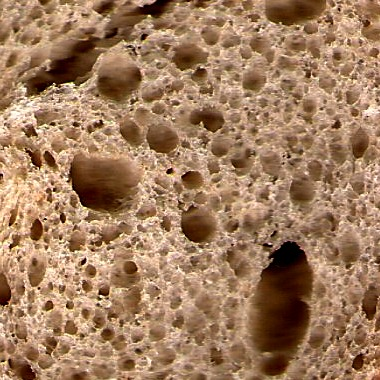
\includegraphics[scale=1]{imagenes/baguette20}
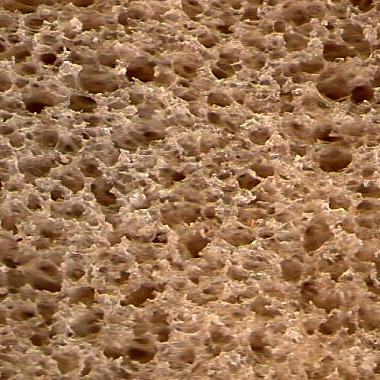
\includegraphics[scale=1]{imagenes/lactal14}
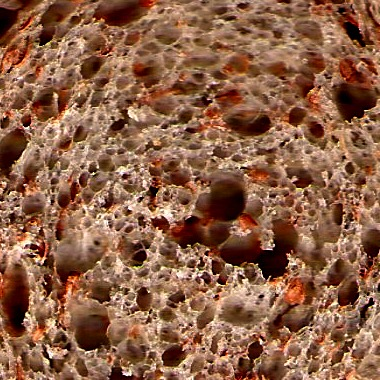
\includegraphics[scale=1]{imagenes/salvado43}
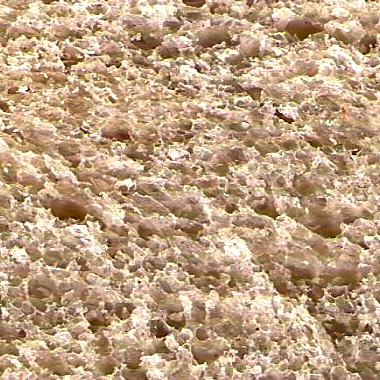
\includegraphics[scale=1]{imagenes/sandwich43}
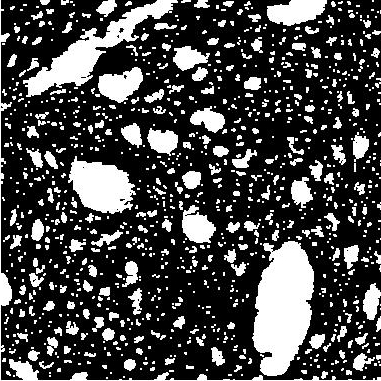
\includegraphics[scale=0.205]{imagenes/baguette20bin}
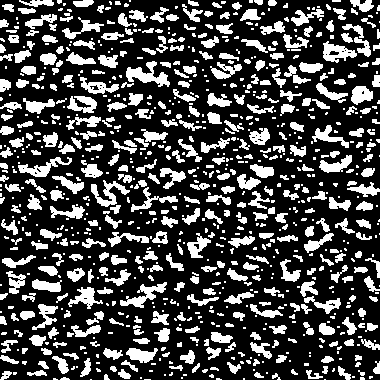
\includegraphics[scale=0.26]{imagenes/lactal14bin}
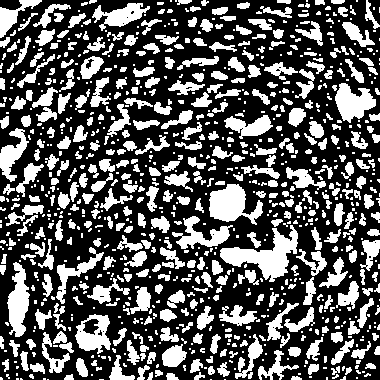
\includegraphics[scale=0.26]{imagenes/salvado43bin}
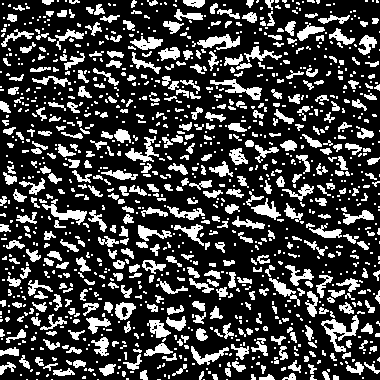
\includegraphics[scale=0.26]{imagenes/sandwich43bin}
\caption{Digitalised images of {\em baguette}, {\em lactal}, {\em salvado} and {\em sandwich} bread types from a scanner with its binarisations}
\label{fig:bread}
\end{figure*}

\begin{figure*}[htb]
\centering
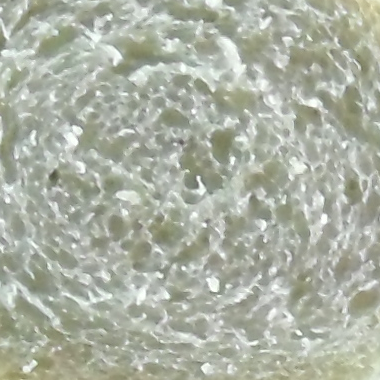
\includegraphics[scale=0.20]{imagenes/b}
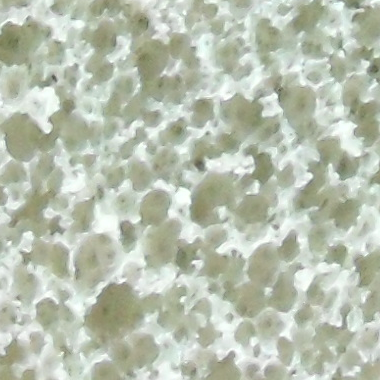
\includegraphics[scale=0.20]{imagenes/l19}
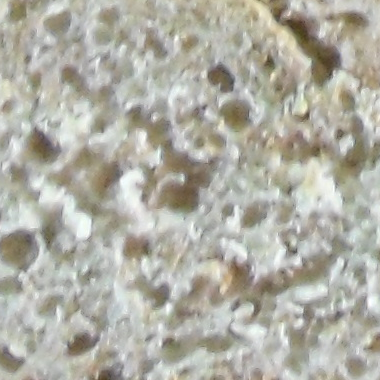
\includegraphics[scale=0.20]{imagenes/s7}
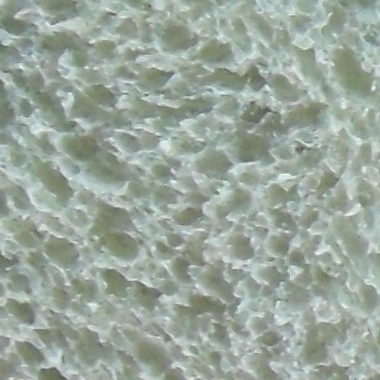
\includegraphics[scale=0.20]{imagenes/Sa14}
\caption{Digitalised images from a digital camera}
\label{fig:camera}
\end{figure*}

\begin{figure*}[htb]
\centering
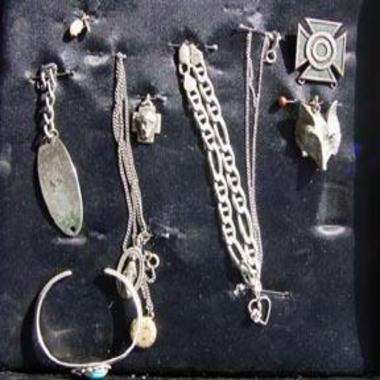
\includegraphics[scale=0.20]{imagenes/image_0036}
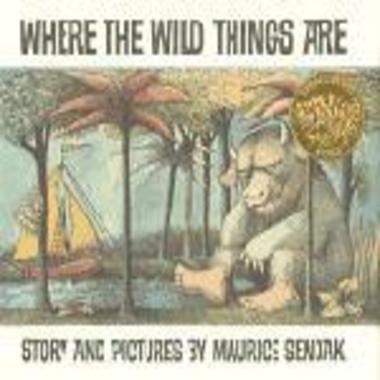
\includegraphics[scale=0.20]{imagenes/image_0041}
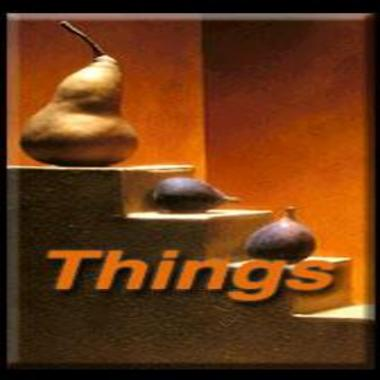
\includegraphics[scale=0.20]{imagenes/image_0042}
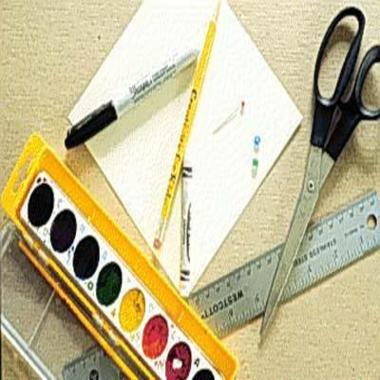
\includegraphics[scale=0.20]{imagenes/image_0048}
\caption{Images from the dataset CalTech101}
\label{fig:nonbread}
\end{figure*}

For the binarisation of the images, the algorithm presented in \cite{White83} was used. This algorithm applies a local thresholding schema, which showed better results than using a global thresholding schema. Particularly, the algorithm presented in \cite{Huang95} and used in \cite{Gonzales2008}, showed poor results when the illumination conditions vary. In Fig.~\ref{fig:bread} an image of each bread type used in this work (top row) and its resulting binarisation using the proposed algorithm (bottom row) is shown.  

\subsection{Feature vectors}

Following the ideas presented in \cite{Gonzales2008}, the mentioned multifractal features were obtained for each image. The code of the algorithms for the computation of the sandbox method was written and run in python. The actual implementation of the method takes approximately two seconds per image to run, and does not depend in the image size (since it depends in the number of points used in the average).

\section{Results}

\subsection{Classification}
{\em Support Vector Machines} (SVM)~\cite{Boser92} were used to perform the classification, using the {\em libsvm}~\cite{Chang2011} implementation. The method of {\em k-fold cross validation} was employed in order to validate the results with $k = 4$, {\em i.e.}, $75\%$ of samples are used as training and $25\%$ as testing (then switching the training and testing samples). The cross validation is applied only to scanner samples.

A robust bread crumb classifier could be used to make the classification process independent of the image capturing condition. In each case, we performed a test in order to show the accuracy of the classifiers when there is a capturing condition mismatch between training and testing samples, {\em i.e.}, when training with scanner samples and testing with camera samples. Based on the randomness in the method's point selection, we made an {\em ensemble} of $10$ trained SVMs models, in which each SVM prediction {\em votes} for one bread type. Then the most appearing class (the most voted class for each image) is selected in each case. In the case of cross validation, we made an average of the percentages obtained. Table \ref{table:tableFirstTest} shows classification results for the classifier when varying different parameters of the method.

\begin{table}[htb]
\centering
\begin{tabular}{|c|c|c|c|c|c|}
    \hline
    \# Fractal Dimensions & $14$ & $8$ & $20$ & $20$ & $30$\\
    \hline
    $R_{max}$ & $40$ & $20$ & $20$ & $20$ & $20$\\
    \hline
    \# Points & $900$ & $900$ & $900$ & $2500$ & $900$\\
    \hline
    Cross Validation  & $75,5\%$ & $76,2\%$ & $77,1\%$ & $79,8\%$ & $77,4\%$\\
    \hline
    Robustness & $46\%$ & $44\%$ & $49\%$ & $49\%$ & $47\%$ \\
    \hline
\end{tabular}
\caption{Results obtained with different parameters}
\label{table:tableFirstTest}
\end{table}

%\begin{table}[htb]
%\centering
%\begin{tabular}{|c|c|c|c|c|}
%    \hline
%    \# Fractal Dimensions & $14$ & $14$ & $14$ & $14$ \\
%    \hline
%    $R_{max}$ & $10$ & $18$ & $30$ & $40$ \\
%    \hline
%    \# Points & $1500$ & $1500$ & $1500$ & $1500$ \\
%    \hline
%   Accuracy  & $78\%$ & $73\%$ & $77\%$ & $77\%$ \\
%    \hline
%    Robustness & $32\%$ & $51\%$ & $\textbf{56\%}$ & $49\%$\\
%    \hline
%\end{tabular}
%\caption{Results obtained with different $R_{max}$}
%\label{table:tableSecondTest}
%\end{table}


%\begin{table}[htb]
%\centering
%\begin{tabular}{|c|c|c|c|c|c|c|c|}
%    \hline
%    \# Fractal Dimensions & $14$ & $14$ & $14$ & $14$ & $14$ & $14$ & $14$ \\
%    \hline
%    $R_{max}$ & $30$ & $30$ & $30$ & $30$ & $30$ & $30$ & $30$ \\
%    \hline
%    \# Points & $100$ & $300$ & $900$ & $1500$ & $2500$ & $3500$ & $4900$\\
%    \hline
%    Accuracy  & $64\%$ & $74\%$ & $77\%$ & $77\%$ & $80\%$ & $85\%$ & $79\%$ \\
%    \hline
%    Robustness & $40\%$ & $45\%$ & $54\%$ & $\textbf{56\%}$ & $44\%$ & $54\%$ & $\textbf{56\%}$\\
%    \hline
%\end{tabular}
%\caption{Results obtained varying the amount of points}
%\label{table:tableThirdTest}
%\end{table}

In Table \ref{table:ConfusionMatrixFractal} the confusion matrix of the data using the classifier in the robustness test is shown. The matrix shows that the classifier tends to label most of the data to the non-bread class. It also shows that the {\em baguette} bread type is successfully discriminated.
\begin{table}[htb]
\centering
\begin{tabular}{|c|c|c|c|c|c|}
    \hline
    Classes & {\em baguette} & {\em lactal} & {\em salvado} & {\em sandwich} & non bread\\
    \hline
    \hline
    {\em baguette}  & $20$ & $0$ & $0$ & $0$  & $0$\\
    \hline
    {\em lactal}    & $1$ & $1$ & $0$ & $0$  & $18$\\
    \hline
    {\em salvado}   & $0$ & $3$ & $2$ & $0$  & $15$\\
    \hline
    {\em sandwich}  & $0$ & $4$  & $0$ & $0$ & $16$\\
    \hline
    non bread       & $1$ & $0$  & $0$ & $0$  & $19$\\
    \hline
\end{tabular}
\caption{Confusion Matrix for the multifractal features}
\label{table:ConfusionMatrixFractal}
\end{table}

It can be seen that the values for the cross validation and for the robustness tests are similar when varying the parameters of the method. In a previous work \cite{Baravalle2012b}, we found similar results for robustness ($50\%$) but a higher accuracy in the cross validation of the scanned images ($93.2\%$), using the singularity multifractal spectrum. We conclude that the sandbox multifractal method performs similarly to the singularity multifractal spectrum.

\section{Conclusions}
The use of multifractal features in bread crumb texture classification showed good performance. The sandbox multifractal spectrum demonstrated to be accurate enough to perform a classification of different bread types. A combination of both multifractal methods could lead to a stronger classifier. The use of boosting could improve the robustness of the method.

The results found can be applied to validate synthetic samples, {\em i.e.}, the latter should have similar features to the bread type that is trying to simulate. These results can be extended to be used as quality parameters for these products. The robustness of the method needs to be enhanced. It will be useful to apply a Principal Component Analysis in order to identify the key variables in the feature vectors. 


\bibliography{bibliografia/bib}
\bibliographystyle{unsrt}
\end{document}
